\documentclass[a4paper,12pt]{article}
\usepackage[utf8]{inputenc}
\usepackage{fancyhdr}
\usepackage{enumitem}
\usepackage{hyperref}
\usepackage{natbib}
\usepackage[french]{babel}

\setlength{\parindent}{1cm}
\usepackage{mwe,lipsum}
\usepackage[section]{placeins}
\usepackage{dblfloatfix}
\usepackage{float}
\usepackage[utf8]{inputenc}
\usepackage[T1]{fontenc}
\usepackage{graphicx}
\usepackage{fullpage}
\usepackage{eso-pic}
\usepackage{layout}
\usepackage{indentfirst}
\usepackage{siunitx}
\usepackage{amsmath}
\usepackage{amssymb}
\usepackage{tabularx}
\usepackage{multicol}
\usepackage{multirow}

\usepackage{caption}
\usepackage{subcaption}

\setlength{\headsep}{0.3cm}
\renewcommand*\contentsname{Table des matières}

\begin{document}
	\pagestyle{fancy}
	\headheight=15pt
	\fancyhf{}
	\renewcommand{\footrulewidth}{0.4pt}
	
	\lhead{DNS over HTTPS}
	\rhead{IP}
	% \lfoot{Equipe 9 - 2020}
	\rfoot{\thepage}
	
	%   TITLE PAGE
	\begin{titlepage}
		
		\begin{center}
			\rule{\textwidth}{1pt} % Thick horizontal rule
			
			\vspace{2pt}\vspace{-\baselineskip} % White space between rules
			
			\rule{\textwidth}{0.4pt} % Thin horizontal rule
			
			\vspace{0.1\textheight} % White space between the top rules and title
			
			%------------------------------------------------
			%	Title
			%------------------------------------------------
			
			\textcolor{black} {
				{\Huge DNS over HTTPS}\\[0.5\baselineskip]
			}
			
			\vspace{0.01\textheight} % White space between the title and short horizontal rule
			
			\rule{0.3\textwidth}{0.4pt} % Short horizontal rule under the title
			
			\vspace{0.1\textheight}
			
			%------------------------------------------------
			%	Author
			%------------------------------------------------
			
			{\Large \textsc{Arnaud Lombardi - Théo Grosperrin}} % Author name
			
			\vspace{0.025\textheight}
			
			{\large \textsc{\today}}
			
			\vfill % White space between the author name and publisher
			
		\end{center}
		
		%------------------------------------------------
		%	Publisher
		%------------------------------------------------
		
		\centering
		{
\includegraphics[scale=0.5]{Images/INSA_LOGO.png}}\\[1.7\baselineskip]
		{
\includegraphics[scale=0.18]{Images/TC.jpg}}
		
		\vspace{0.1\textheight} % White space under the publisher text
		
		%------------------------------------------------
		%	Bottom rules
		%------------------------------------------------
		
		\centering
		
		\rule{\textwidth}{0.4pt} % Thin horizontal rule
		
		\vspace{2pt}\vspace{-\baselineskip} % White space between rules
		
		\rule{\textwidth}{1pt} % Thick horizontal rule
		
	\end{titlepage}
	
	% Front matter %
	\setcounter{page}{1}
	\pagenumbering{arabic}
	
	%------------------------------------------------
	%	Table of contents
	%------------------------------------------------
	\hspace{2cm}
	\tableofcontents
	
	\newpage
	
	\section{En quelques mots, qu'est que le DoH ?}
	Il s'agit de la résolution des requêtes DNS en utilisant le protocole HTTPS, au lieu de simples requêtes en clair sur le port 53 (DNS classique). L'objectif de cette méthode est d'augmenter la sécurité du cote utilisateur : cela permet d'améliorer la vie privée de l'utilisateur (le trafic entre le client et le serveur DNS est chiffré, illisible par les machines se trouvant sur le chemin), et d'éviter les attaques de type "man-in-the-middle".
	
	\section{Détails techniques}
	Le DoH est un standard publié par l'IETF : \href{https://tools.ietf.org/html/rfc8484}{RFC 8484}.
	
	\subsection{Le fonctionnement du DNS et ses limites}
	DNS est un acronyme qui signifie « Domain Name System » et peut se traduire par « système de noms de domaine ».
	Le DNS est un service permettant de faire le lien entre les noms de domaines et les adresses IP qui leurs sont associées.(ex : google.fr = 216.58.198.195) 
	Pour cela DNS a besoin de plusieurs serveurs pour répondre au requête DNS des utilisateurs 
	le serveur DNS récursif répond à une requête DNS et demande l’adresse à d’autres serveurs DNS,  le serveur TLD (top-level domain : domaine de premier niveau) est l’un des serveurs DNS de haut niveau que l’on trouve sur Internet, le serveur de noms faisant autorité constitue le terminus d’une requête DNS et les serveur racine du DNS (Root Name Server) : il s’agit du serveur de noms pour la zone racine. Il répond à des requêtes directes et peut renvoyer une liste de noms de serveurs faisant autorité pour le domaine de haut niveau correspondant.
	\begin{figure}[H]
		\begin{center}
			{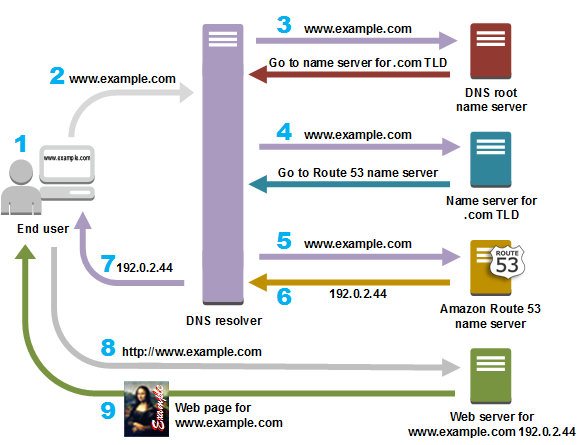
\includegraphics[scale=0.6]{Images/routes-traffic.png}}
		\end{center}
		\caption{Schéma d'une requête DNS.}
	\end{figure}
	Une requête consiste à envoyer sur le port 53 une requête en clair de type adresse « A » pour récupérer l’IP en passant par les diffèrent serveur 
	
	Limite :
	DNS utilise en général UDP et le port 53. La taille maximale des paquets utilisée est de 512 octets. Si une réponse dépasse cette taille, la norme prévoit que la requête doit être renvoyée sur le port TCP 53. Ce cas est cependant rare et évité, et les firewalls bloquent souvent le port TCP 53. Les transferts de zone s'effectuent par TCP sur le même numéro de port. Pour des raisons de sécurité, les serveurs restreignent généralement la possibilité de transférer des zones.
	
	Plusieurs faille de DNS sont connu dû au fait que les requête soit envoyer en clair : 
	Une des failles mises en avant est la possibilité d'intercepter les paquets transmis. Les serveurs DNS communiquent au moyen de paquets uniques et non signés. Ces deux spécificités rendent l'interception très aisée. L'interception peut se concrétiser de différentes manières, notamment via une attaque de type « man in the middle », de l'écoute des données transférées et de l'envoi de réponse falsifiée
	Les paquets des serveurs DNS étant faiblement sécurisés, authentifiés par un numéro de requête, il est possible de fabriquer de faux paquets. Par exemple, un utilisateur qui souhaite accéder au site http://mabanque.example.com fait une demande au site DNS. Il suffit, à ce moment, qu'un pirate informatique réponde à la requête de l'utilisateur avant le serveur DNS pour que l'utilisateur se retrouve sur un site d'hameçonnage.
	La trahison par un serveur, ou corruption de données, est, techniquement, identique à une interception des paquets. La seule différence venant du fait que l'utilisateur envoie volontairement sa requête au serveur. Cette situation peut arriver lorsque, par exemple, l'opérateur du serveur DNS souhaite mettre en avant un partenaire commercial.
	L'empoisonnement du cache DNS ou pollution de cache DNS (en anglais, DNS cache poisoning) est une technique permettant de leurrer les serveurs DNS afin de leur faire croire qu'ils reçoivent une requête valide tandis qu'elle est frauduleuse.
	Une attaque par déni de service (ou attaque par saturation; en anglais, Denial of Service attack ou DoS attack) est une attaque sur un serveur informatique qui résulte en l'incapacité pour le serveur de répondre aux requêtes de ses clients.
	
	\subsection{Le fonctionnement du DoH}
	
	\section{Les différentes implémentations typiques}
	
	\subsubsection{DoH natif au sein du navigateur}
	
	C'est la méthode à privilégier, mais aussi la plus complexe à mettre en place : l'application effectue elle-même une requête DoH, elles n'ont donc pas besoin de passer par la fonction DNS du système d'exploitation. Les désavantages de cette implémentation restent multiples : l'application peut ne pas informer l'utilisateur qu'elle effectue ou non la requête de manière sécurisée (par exemple, si elle ne le supporte pas, elle n'en informera probablement pas l'utilisateur). De plus, cela demande une mise à jour de chaque application afin de la rendre compatible DoH de manière native.
	
	\begin{figure}[H]
		\begin{center}
			{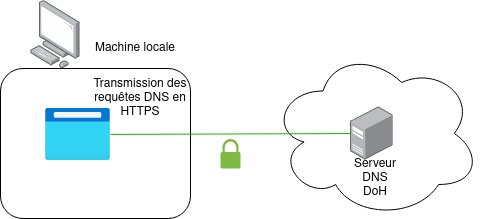
\includegraphics[scale=0.6]{Images/schema_doh_native.png}}
		\end{center}
		\caption{Schéma de l'implémentation native de DoH au sein d'une application.}
	\end{figure}
	 
	
	\subsubsection{Proxy DoH sur le réseau local}
	
	Dans ce scénario, les machines du réseau local effectuent des requêtes DNS traditionnelles sur le port 53, vers un serveur DNS installé sur le réseau local. Ce serveur DNS effectue ensuite une requête DNS récursive vers un serveur DNS compatible DoH. Ainsi, la requête est chiffrée lorsqu'elle sort du LAN.
	
	\begin{figure}[H]
		\begin{center}
			{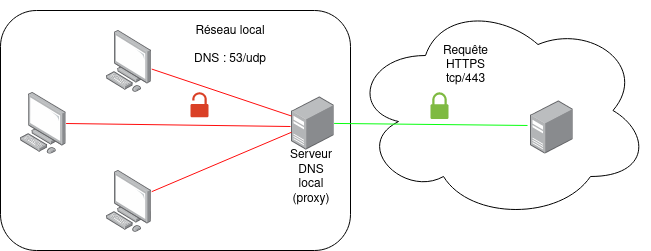
\includegraphics[scale=0.6]{Images/schema_doh_proxy_lan.png}}
		\end{center}
		\caption{Schéma de l'implémentation d'un serveur DoH proxy sur un réseau local.}
	\end{figure}
	
	On constate bien l'inconvénient de ce système : les requêtes entre les clients et le serveur local ne sont pas sécurisées, et on se base sur le fait que l'on fait confiance au serveur proxy.
	Cependant, il s'agit d'un méthode d'implémentation relativement facile à mettre en place, puisqu'elle n'implique que peu de modifications sur le réseau existant, simplement l'ajout d'un proxy sur le LAN.
	
	\subsubsection{Proxy DoH sur système local}
	
	Ici, le système est configuré pour envoyer les requêtes DNS à lui-même, puisqu'on installe un serveur proxy sur celui-ci. Ce proxy se charge d'effectuer les requêtes de manière sécurisée (donc DoH) pour chaque requête DNS classique qu'il reçoit.
	Cette méthode permet d'utiliser des applications n'implémentant pas le DoH de manière native sans compromettre la sécurité des requêtes sur le LAN. Cependant, elle est lourde puisqu'elle implique d'installer un proxy sur chaque machine.
	
	\begin{figure}[H]
		\begin{center}
			{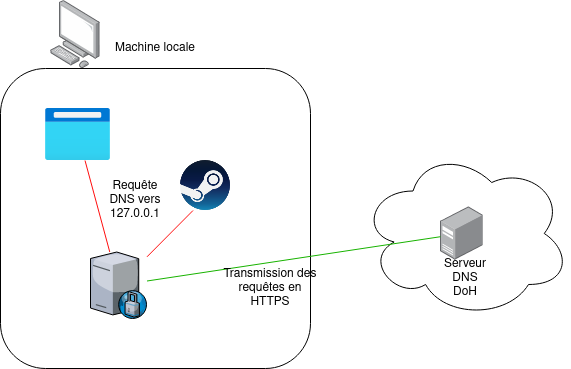
\includegraphics[scale=0.6]{Images/schema_doh_proxy_local.png}}
		\end{center}
		\caption{Schéma de l'implémentation d'un serveur proxy DoH sur le système local.}
	\end{figure}

	\section{Mise en contexte}
	
	\subsection{Support logiciel}
	
	\subsubsection{Système d'exploitation}
	DoH est implémenté sur Windows 10 depuis la version 19628 (mai 2020), iOS 14 et macOS 11 depuis fin 2020. Le support est donc très récent (et donc restreint).
	\subsubsection{Navigateurs compatibles}
	Les navigateurs les plus populaires sont compatibles DoH :
	\begin{itemize}
		\item Mozilla Firefox : suite à un partenariat avec Cloudflare, l'option est disponible des 2018. Depuis le 25 février 2020, Firefox active le DoH par défaut pour tous les utilisateurs des Etats-Unis.
		\item Google Chrome : disponible depuis la version 83 pour Windows et macOS, la fonctionnalité est accessible depuis les paramètres du navigateur. En septembre 2020, la version Android du navigateur supporte le DoH.
		\item Microsoft Edge : compatible (le navigateur est un fork de Google Chrome).
	\end{itemize}
	\subsubsection{Serveurs compatibles}
	BIND 9, un serveur DNS open-source et très répandu, a introduit le support du DoH en février 2021, sur la version 9.17.10.
	Quant à Unbound, il le supporte depuis octobre 2020 (version 1.12.0). Il supportait déjà le DoT (DNS over TLS) depuis décembre 2011.
	\subsection{Critiques}
	Le DoH, comme de nombreuses technologies cherchant a améliorer la sécurité, n'a pas manqué d'être le sujet de critiques diverses. En effet, certains pirates ont su tirer profit de ce protocole : en 2019, le ver Godlua, qui a servi à exécuter diverses attaques de type DDoS, a utilisé le DoH afin de masquer la destination de son serveur de contrôle.
	Mais il a également été critiqué par le gouvernement du Royaume-Uni : le pays a mis en place divers filtres afin de bloquer des sites web proposant du contenu illégalement, ou bien l'accès au sites pornographiques (pour lesquels il faut entrer un numéro de carte bancaire afin de prouver la majorité du visiteur dans ce pays). Mozilla a été accusé de "Internet Villain" par l'ISPA (Internet Service Providers Association) pour avoir sapé les standards en matière de sécurité web du Royaume-Uni. Mozilla a été contraint de désactiver par défaut le DoH sur son navigateur pour les utilisateurs anglo-saxons.\href{https://www.theguardian.com/technology/2019/sep/24/firefox-no-uk-plans-to-make-encrypted-browser-tool-its-default}{Source}
	\section{Les problèmes que peuvent poser le DoH}	
	
\end{document}